\section{Introduction}\label{introduction}

\subsection{Motivation}\label{motivation}
The work done in this report is done in cooperation with Sensomar SEALAB.
Sensomar SEALAB is a company developing camera systems for underwater use. Most of this is planned to be used in the fishing industry, especially aimed towards salmon breeding industry. The company's current goal is to be able to automatically measure the size and weight of the salmon underwater. For this goal to be reached, SEALAB uses some of the best cameras available, that has very high resolution and a very accurate depth measurement. But, due to all particles in the water, other fish in the background and light reflections, it is still not possible to use the data directly to find accurate measurements of the fish. They therefore need to both detect the fish, to be able to take a good photo, and they will need quite a bit of image processing on that image to remove all irrelevant data before they can find the measurements of the fish. 

With the use of image processing for noise and particle removal, it is reasonable to believe that the size measurements of the fish could be improved.

This report will show relevant background study with explanations to the different techniques that have been tried out. It will show implementation and results from different approaches. All image processing done throughout this project is done through the use of C++ and OpenCV library. OpenCV (Open Source Computer Vision) is a library of programming functions mainly aimed at real-time computer vision. \cite{website:opencv_wiki}

%%%%%%%%%%%%%%%%%%%%%%%%%%%%%%%%%%%%%%%%%%%%%%%%%%%%%%%%%%%%%%%%%%%%%%

\subsection{Image processing simple intro??}

{\color{red}Add image examples}


%%%%%%%%%%%%%%%%%%%%%%%%%%%%%%%%%%%%%%%%%%%%%%%%%%%%%%%%%%%%%%%%%%%%%%

\subsection{The Raytrix Camera}

\begin{figure}[h]
    \centering
    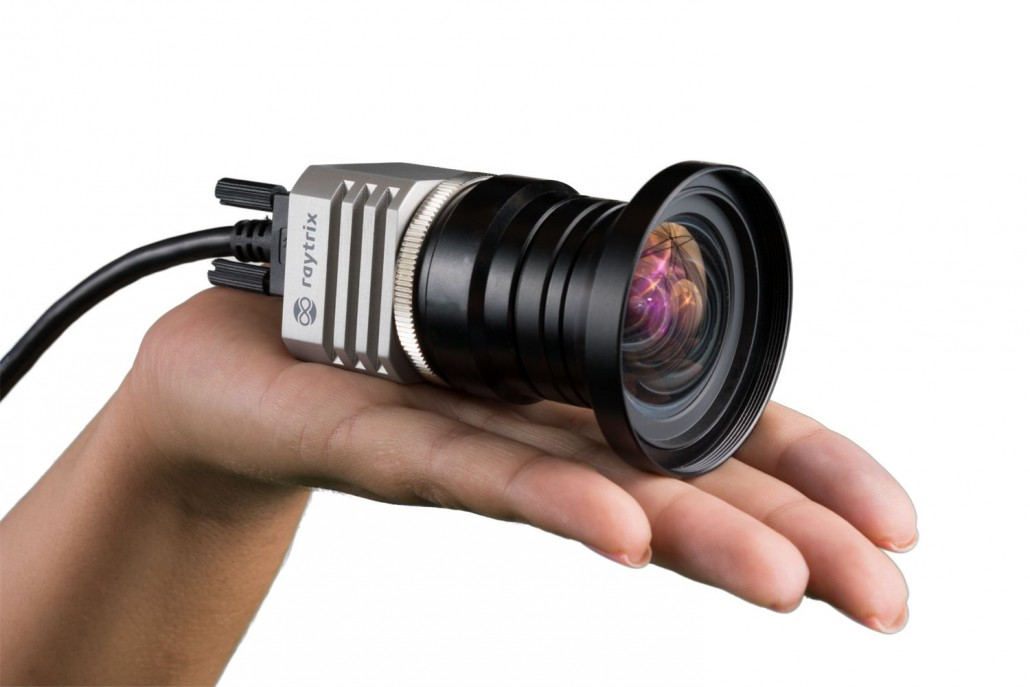
\includegraphics[width=.9\linewidth]{Images/raytrix_camera}
    \caption{Raytrix R42 Camera}
    \label{fig:raytrix_camera}
\end{figure}

The camera used throughout this project is the Raytrix R42 camera. The camera is developed by Raytrix, a German company which offers several 3D Light Field cameras intended for professional and industrial use. The R42 is their highest resolving light field camera to date. It is based on a 42 megaray sensor and offers an effective resolution up to 10 megapixels at 7 FPS. \cite{website:raytrix_r42}

Light Field cameras are a new type of 3D-cameras that capture a standard image together with the depth information of a scene. Metric 3D information can be captured with a single light field camera through a single lens in a single shot using just the available light. Raytrix has specialized on developing light field cameras for industrial applications. A patented micro lens array design allows for an optimal compromise between high effective resolution and large depth of field. Raytrix cameras are already in use in applications like volumetric velocimetry, plant phenotyping, automated optical inspection and microscopy, to name a few. \cite{website:raytrix_main}

This camera is therefore very useful for industrial purposes, as you can get both a clear image, a depth map, and a 3D model of the scene. It has though no documented use underwater, and since the physical properties of water cause degradation effects not present in air, the depth measurements get affected. We get both "holes" in the object, and detected particles in front of the object. If we are going to use this camera technology to measure volume of fish, we need to improve the data received from the camera. Particles in front of the fish needs to be removed, and holes in the fish filled.

The Raytrix camera is build up by a main lens in front, a micro lens array, and the image sensor behind. The micro lens array has many thousand micro lenses, 4000x2600 lenses. The micro lens array is placed in front of the image sensor inside the camera, which turns the image sensor into a micro-camera array (\ref{fig:light_field}), where each micro-camera sees part of the intermediate image from a slightly different perspective. That is, instead of using a large camera array that looks at the object directly, we can choose a main lens to select the desired field-of-view and create the intermediate image in front of the micro camera array. The images generated by the camera in this setup are processed on a PC with appropriate software algorithms to calculate the scene depth and to reconstruct a 2D image. When all processing is done on a GPU, it allows for 30 megapixel 2D and 3D images per second (30 FPS). \cite{website:raytrix_technology}

\begin{figure}[h]
    \centering
    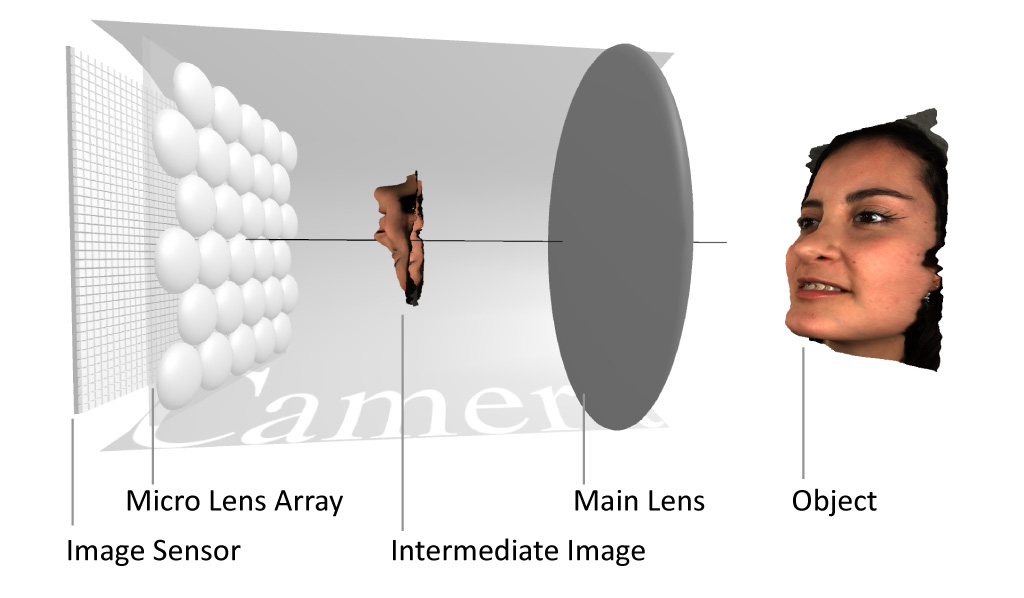
\includegraphics[width=.9\linewidth]{Images/Light-Field-Camera-Schematic}
    \caption{Raytrix Light Field Technology}
    \label{fig:light_field}
\end{figure}

When calibrating the camera the raw image is used to make sure the main objects edges are shown in several of the micro lenses. The more micro lenses picking up one object, the better the depth measurement. 

The raw image shows the capture from all micro lenses, as seen in figure \ref{fig:raw_image}. The camera perform no processing internally, it simply deliver a raw image to a PC, which is then processed on a GPU to obtain the 2D and 3D data. 
The totalfocus image - which is just a normal color image - is made from the raw image on a computer, figure \ref{fig:totalfocus}. 
The depthmap, figure \ref{fig:depthmap}, is computed from the raw image, and the 3D image, figure \ref{fig:3d_image}, is made from the depthmap and the totalfocus image. 
The depth in the depthmap is represented by colors, where red is close to the camera, yellow and green is the object centered during calibration, blue is behind the object, and black has no depth. This means that the optimal depthmap image would be all black, with a yellow and green fish.

\begin{figure}[h]
    \centering
    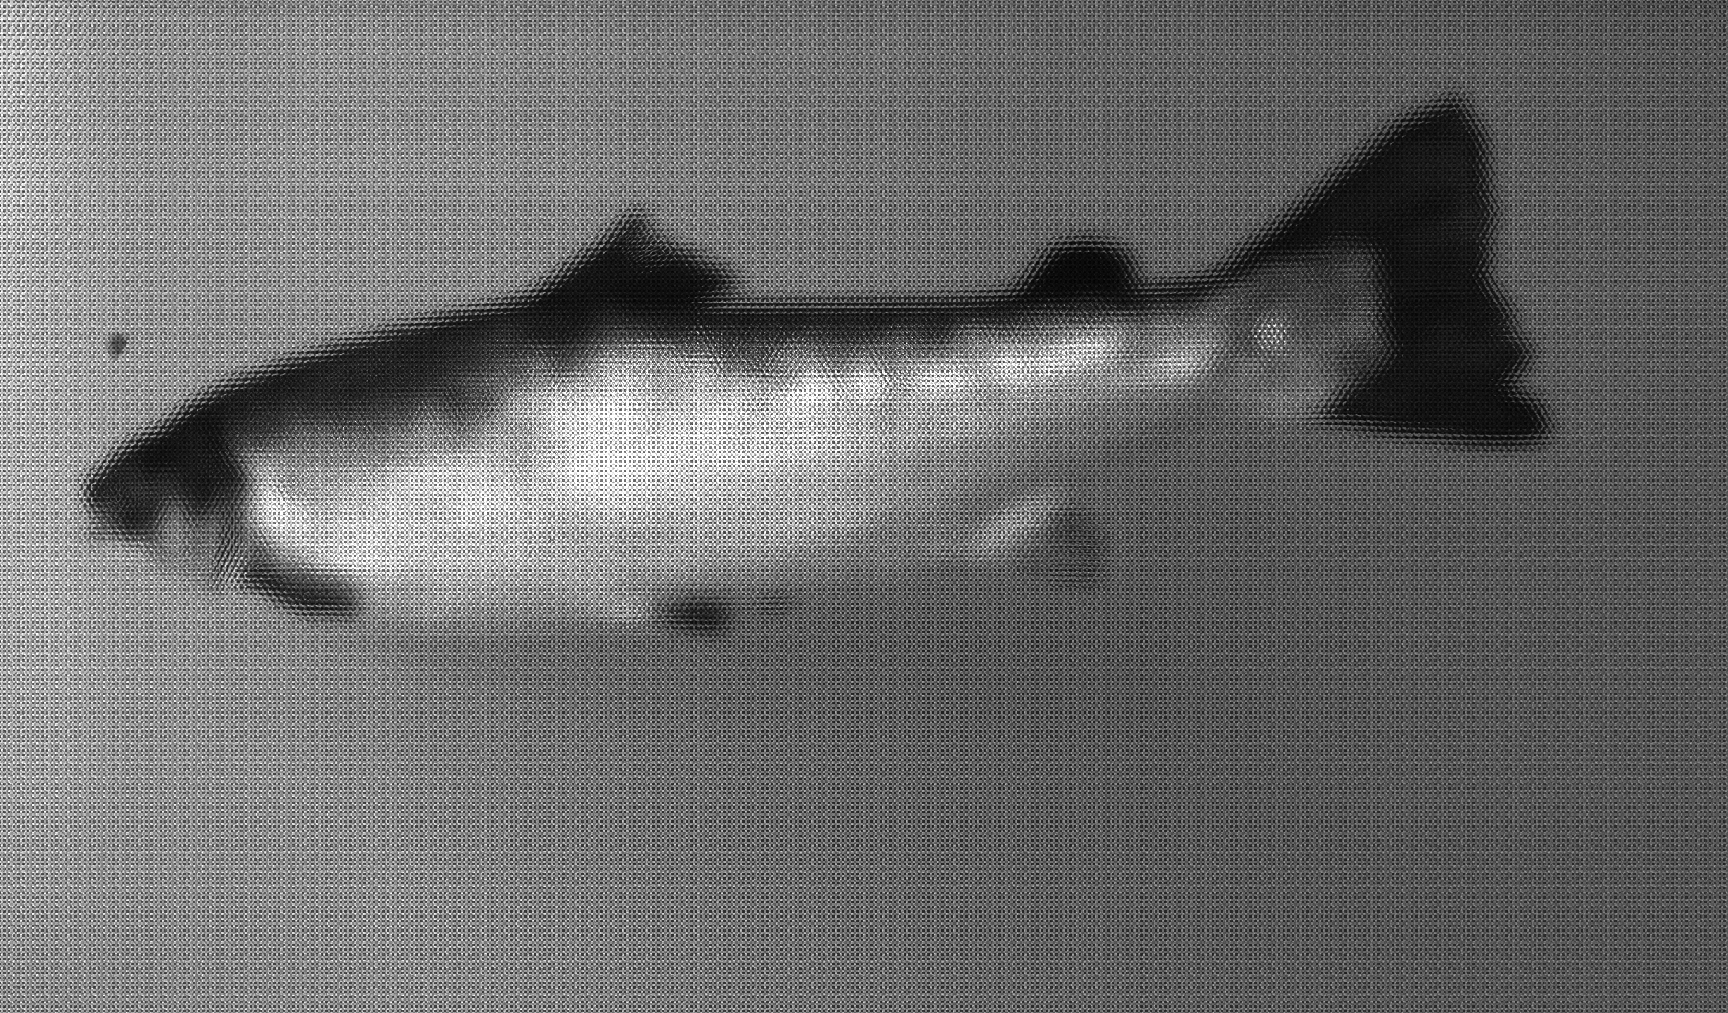
\includegraphics[width=.9\linewidth]{Images/raw}
    \caption{Raw image}
    \label{fig:raw_image}
\end{figure}

\begin{figure}[h]
    \centering
    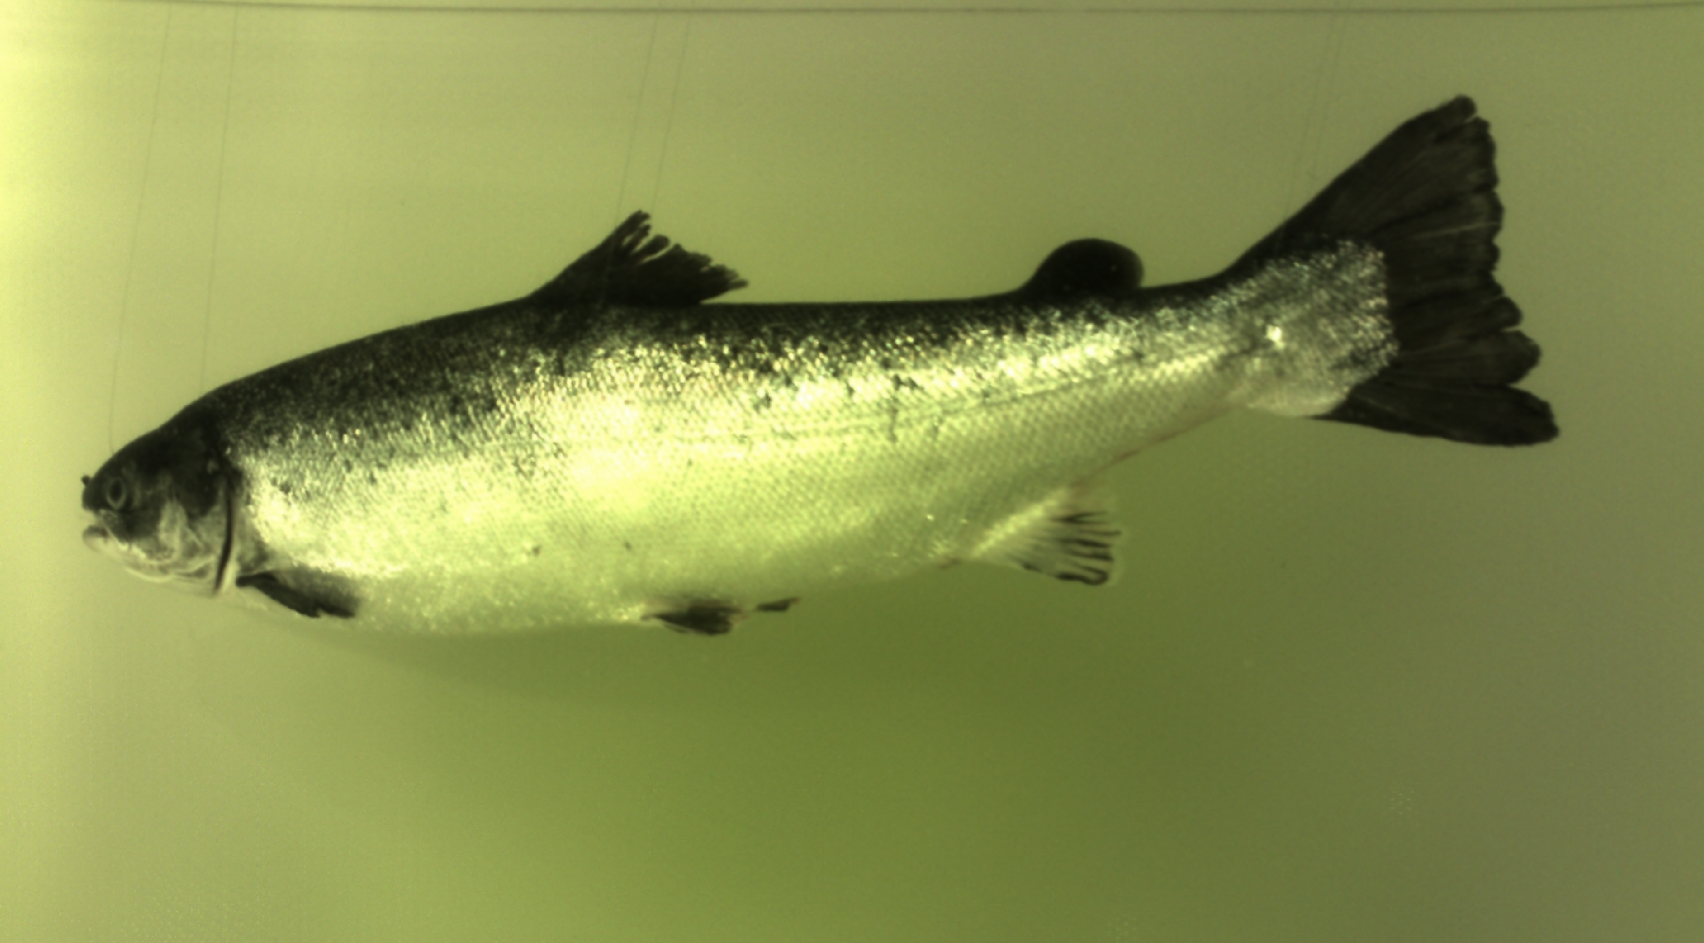
\includegraphics[width=.9\linewidth]{Images/totalfocus}
    \caption{Totalfocus image}
    \label{fig:totalfocus}
\end{figure}

\begin{figure}[h]
    \centering
    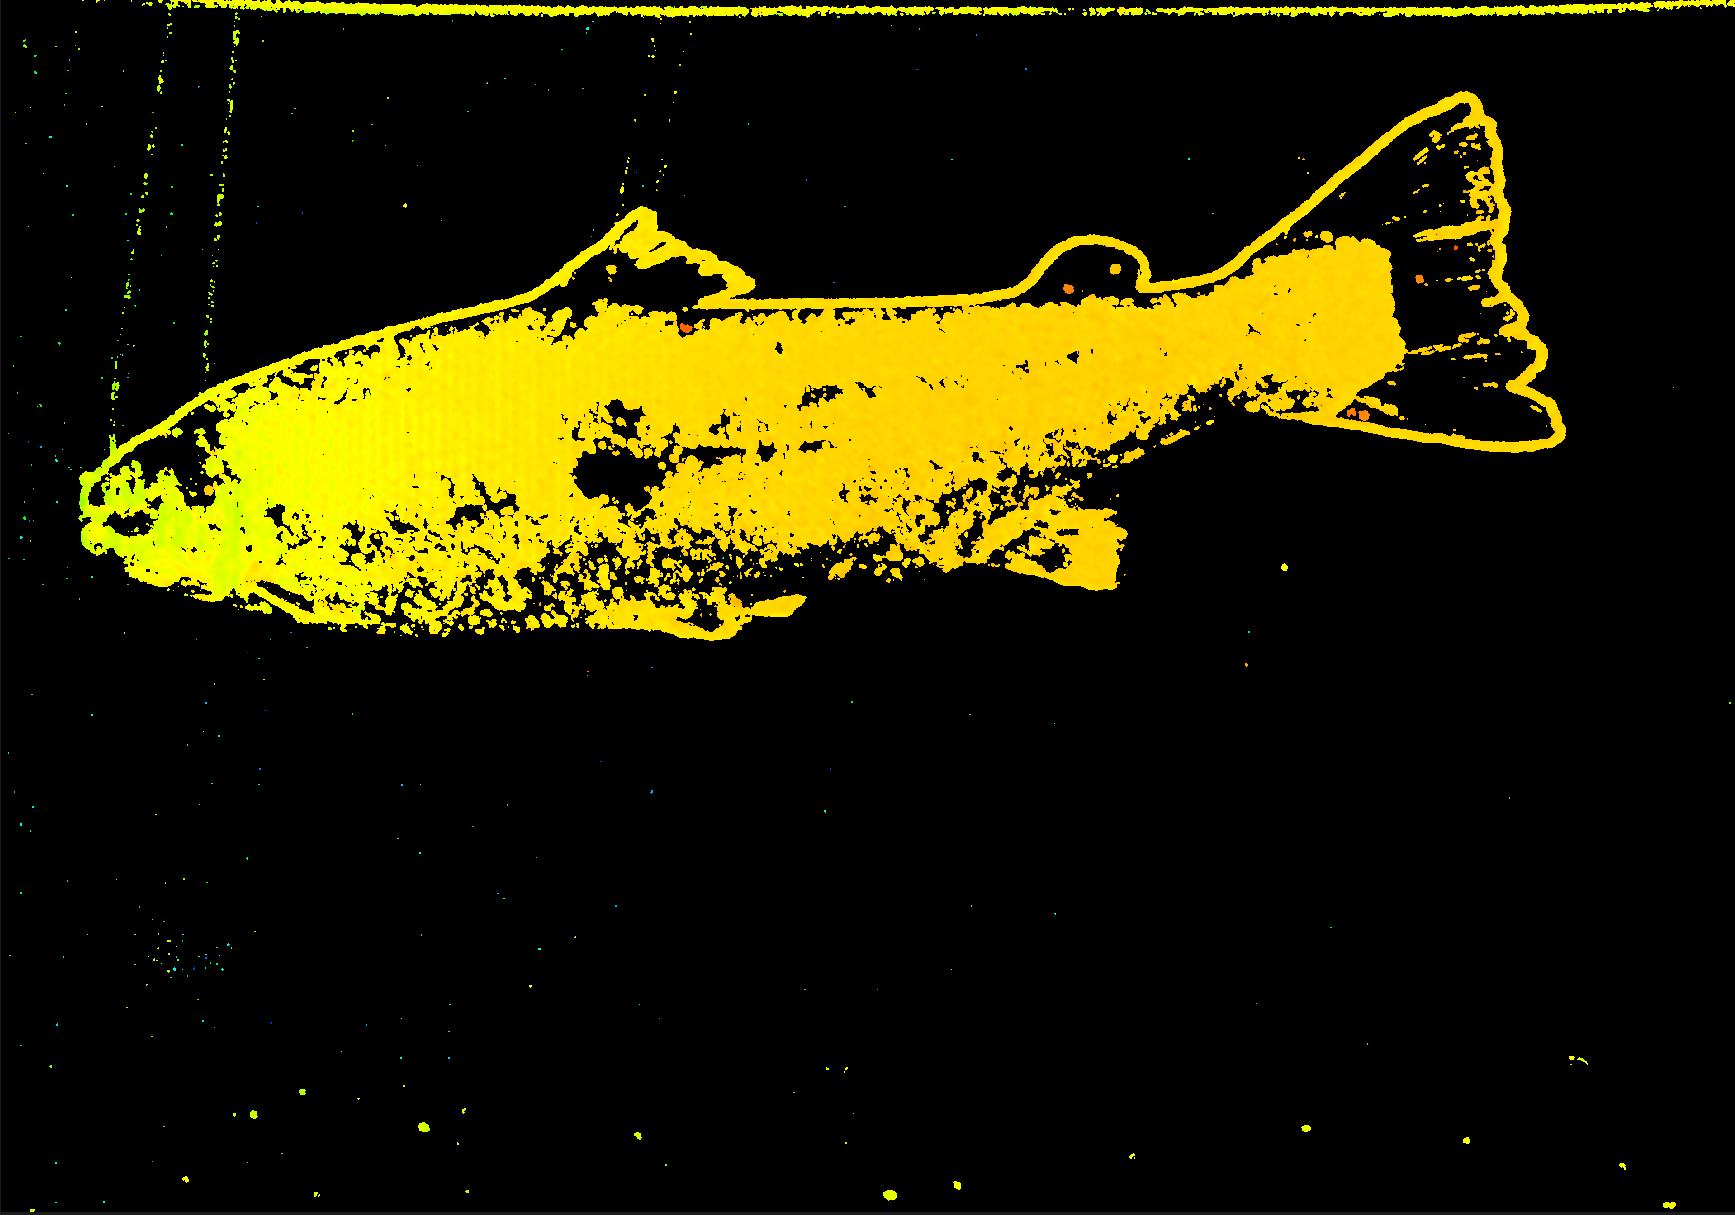
\includegraphics[width=.9\linewidth]{Images/depthmap}
    \caption{Depthmap image}
    \label{fig:depthmap}
\end{figure}

\begin{figure}[h]
    \centering
    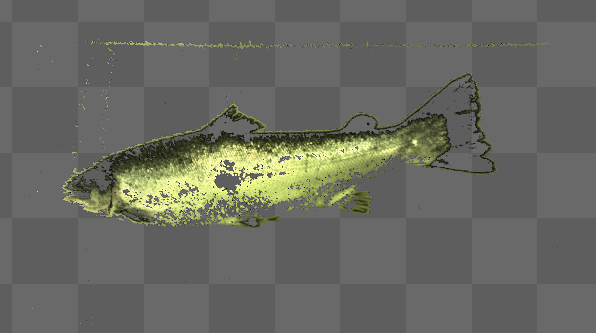
\includegraphics[width=.9\linewidth]{Images/depth3D}
    \caption{3D image}
    \label{fig:3d_image}
\end{figure}

As seen from the 3D image produced in the Raytrix Software, the particles in front will affect the surface of the fish. The same goes for the holes in the fish. What is wanted is a smooth surface of the fish, so that measurements of length, height and thickness is most accurate. Figure \ref{fig:3d_image_side} shows the 3D image in figure \ref{fig:3d_image} turned about 45 degrees to the side. This shows how inaccurate the current 3D model for underwater images are. 
One problem working with the depthmap is that they have their own .ray format. It is not yet possible to do direct image processing using OpenCV on this format, so we therefore convert the depthmap to .png before starting to work on the enhancement.

\begin{figure}[h]
    \centering
    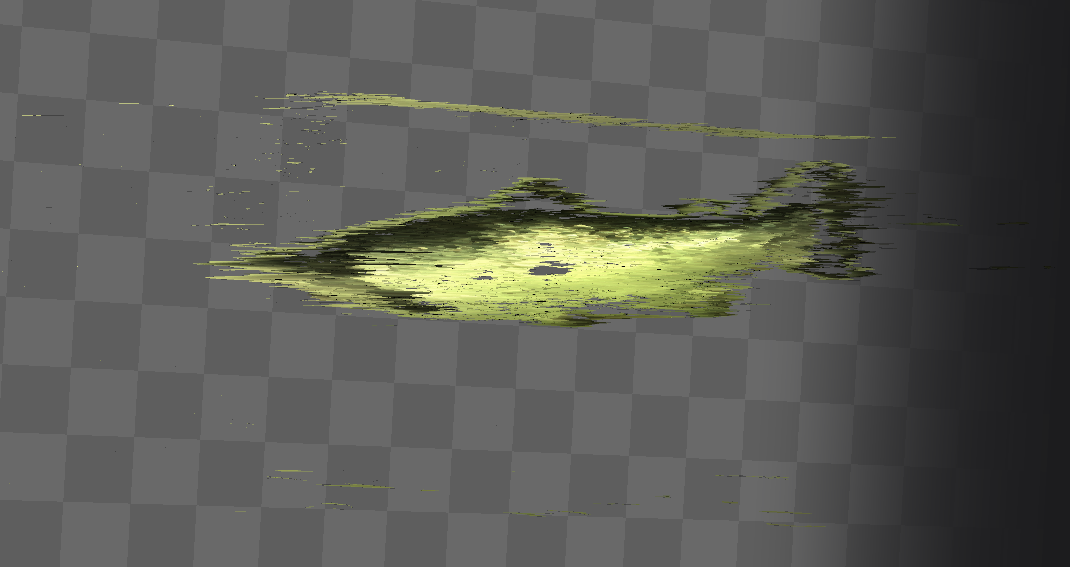
\includegraphics[width=.9\linewidth]{Images/depth3D_side}
    \caption{3D image from the side}
    \label{fig:3d_image_side}
\end{figure}


All images in this subsection is made with the Raytrix software, RxLive 4.0.


{\color{red}Explain more about how the Raytrix measures depth?? Explain the calibration and the RAW image?? And about Light Field Cameras?}
